\documentclass[]{article}
\usepackage[spanish.mexico]{babel}
\usepackage[T1]{fontenc}
\usepackage[utf8]{inputenc}
%\usepackageB.\\{lmodern}
\usepackage[a4paper]{geometry}

%\usepackage{natbib}
\usepackage{cite}


%Grafico de barras
\usepackage{pgfplots}

%Graficos e imagenes
\usepackage{graphicx}


\title{Tarea Cocción}
\author{Pablo Vivar Colina}
%\date{Mayo 2018}



\begin{document}
	
%	%\usepackage[top=2cm,bottom=2cm,left=1cm,right=1cm]{geometry}


\begin{titlepage}
     \begin{center}
	
\includegraphics[width=0.09\textwidth]{UNAM}\Large Universidad Nacional Autónoma de México
        	
\includegraphics[width=0.09\textwidth]{FI}\\[1cm]
        \Large Facultad de Ingeniería\\[1cm]
       % \Large División de Ciencias Básicas\\[1cm]
         \Large Laboratorio de Fundamentos de Control(6655)\\[1cm]
         %la clave antes era:4314
         \footnotesize Profesor: Salcedo Ubilla María Leonor Ing.\\[1cm]
        \footnotesize Semestre 2019-1\\[1cm]
        
       

        \Large Práctica No. 1\\[1cm]
        
           

\Large Introdcción MATLAB
        
         %Texto a la derecha
          \begin{flushright}
\footnotesize  Grupo 2\\[0.5cm]
\footnotesize Brigada: 4\\[0.5cm]
\footnotesize Rodrigo Adrián Martínez López\\[0.5cm]
\footnotesize Vivar Colina Pablo\\[0.5cm]
 \end{flushright}
    %Texto a la izquierda
          \begin{flushleft}
        \footnotesize Ciudad Universitaria Agosto de 2018.\\
          \end{flushleft}
         
          
        %\vfill
        %\today
   \end{center}
\end{titlepage}
 %agregar portada

\maketitle

%\tableofcontents  % Write out the Table of Contents

%\listoffigures  % Write out the List of Figures


\section{Punto de Ebullición}

 Cuando se calienta un líquido, alcanza eventualmente una temperatura en la cual la presión del vapor es lo bastante grande que se forman burbujas dentro del cuerpo del líquido. Esta temperatura se llama punto ebullición. Una vez que el líquido comience a hervir, la temperatura permanece constante hasta que todo el líquido se ha convertido a gas.\\

El punto ebullición normal del agua es 100 $[^oC]$ a una atmósfera de presión. Pero si se trata de cocinar un huevo en agua hirviendo mientras se acampa en la montañas rocallosas a una elevación de 10,000 pies sobre el nivel del mar, usted encontrará que se requiere de un mayor tiempo de cocción ya que el agua hierve a no más de 90 $[^oC]$. Usted no podrá calentar el líquido por encima de esta temperatura a menos que utilice una olla de presión. En una olla de presión típica, el agua puede seguir siendo líquida a temperaturas cercanas a 120 $[^oC]$ y el alimento se cocina en la mitad del tiempo normal.\\

Para explicar porqué el agua hierve a 90 $[^oC]$ en las montañas, o porqué hierve a 120 $[^oC]$ en una olla de presión, aunque su punto ebullición normal es 100 $[^oC]$, primero necesitamos entender porqué los líquidos bullen. Debe quedar claro que se tiene la ebullición de un líquido cuando la presión del vapor del gas que se escapa del líquido es igual a la presión ejercida en el líquido por sus alrededores, según lo muestra la figura \ref{curvaEb}.\\

\begin{figure}[h!]
	\centering
	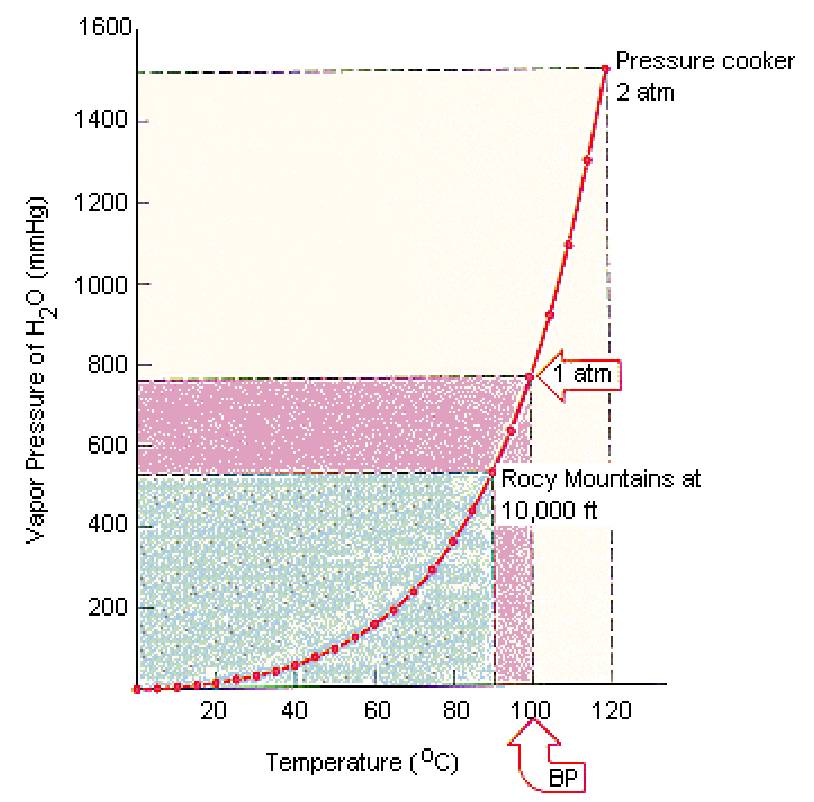
\includegraphics[width=0.3\textwidth]{curvaEb}
    \caption{Curva de Ebullición }
    \label{curvaEb}
\end{figure}

 El punto de ebullición normal del agua es 100 $[^oC]$ porque ésta es la temperatura a la cual la presión del vapor del agua es 760 mmHg, o 1 atmósfera. Es decir que bajo condiciones normales, cuando la presión de la atmósfera es aproximadamente 760 mmHg, el agua tiene un punto de ebullición de 100 $[^oC]$. A 10,000 pies sobre nivel del mar, la presión de la atmósfera es solamente 526 mmHg. A esta presión el punto de ebullición del agua ocurre a una temperatura de 90 $[^oC]$.\\

Las ollas de presión se equipan con una válvula que permite escapar al gas cuando la presión dentro de la olla excede un cierto valor fijo. Esta válvula tiene comúnmente un valor fijo de 15 psi, que significa que el vapor de agua dentro de la olla debe alcanzar una presión de 2 atmósferas antes de que pueda escaparse. Ya que el agua no alcanza una presión de vapor de 2 atmósferas hasta que alcanza la temperatura de 120 $[^oC]$, la temperatura de ebullición dentro del recipiente es de 120 $[^oC]$. \cite{ebullicion}\\

\section{ Tiempo de cocción de los frijoles en olla convencional}


El tiempo de cocción de los frijoles en olla convencional podrá variar dependiendo de la cantidad que estés preparando y de si los mismos van acompañados de carne o únicamente de vegetales. El tiempo de cocción para 250 gramos de frijoles es de 1 hora aproximadamente, mientras que si preparas medio kilo tardará cerca de 2 horas.\\

Es importante que durante la preparación vayas añadiendo agua o caldo para evitar que los frijoles se sequen. A partir de los 45 minutos al fuego ya podrás ir probando las legumbres para asegurarte que las mismas estén completamente suaves antes de sacarlas.\cite{coccion}\\





\section{Referencias}

%\bibliographystyle{plain}
%\bibliography{Prac1}



\begin{thebibliography}{9}
	%\bibitem{latexcompanion} 
	%Michel Goossens, Frank Mittelbach, and Alexander Samarin. 
	%\textit{The \LaTeX\ Companion}. 
	%Addison-Wesley, Reading, Massachusetts, 1993.
	
	%\bibitem{einstein} 
	%Albert Einstein. 
	%\textit{Zur Elektrodynamik bewegter K{\"o}rper}. (German) 
	%[\textit{On the electrodynamics of moving bodies}]. 
	%Annalen der Physik, 322(10):891–921, 1905.
	
	
	\bibitem{ebullicion} 
	 Punto ebullición,
	\\\texttt{http://www.cie.unam.mx/~ojs/pub/Liquid3/node8.html}
	
	
	\bibitem{coccion} 
   UnComo:Tiempo de cocción de los frijoles,
	\\\texttt{https://comida.uncomo.com/articulo/tiempo-de-coccion-de-los-frijoles-34777.html}
\end{thebibliography}






\end{document}
